\subsection{2-d results}
Optigrid settings: 4 Clusters, Cluster size = [10000, 20000, 20000, 20000], Noise samples of 1000, $kde\_bandwidth$ of 0.2, $noise\_level$ of 0.1, and max cut score of 1

\begin{tcolorbox}
\small
Cluster 0: Mean=[-5.31 -4.93], Std=[2.19 2.39]\newline
Cluster 1: Mean=[-1.42e-03  4.87e+00], Std=[1.00 1.57]\newline
Cluster 2: Mean=[ 5.17 -0.09], Std=[1.76  1.93]\newline
Cluster 3: Mean=[-6.90 19.97], Std=[2.06 1.08 ]
\end{tcolorbox}
\normalfont

The OptiGrid algorithm did a reasonable job of clustering the data. 
The clusters are well separated and the noise is minimal. 
The clusters are not perfectly circular, but the algorithm was able to capture the general shape of the clusters.

\begin{figure}[H]
    \centering
    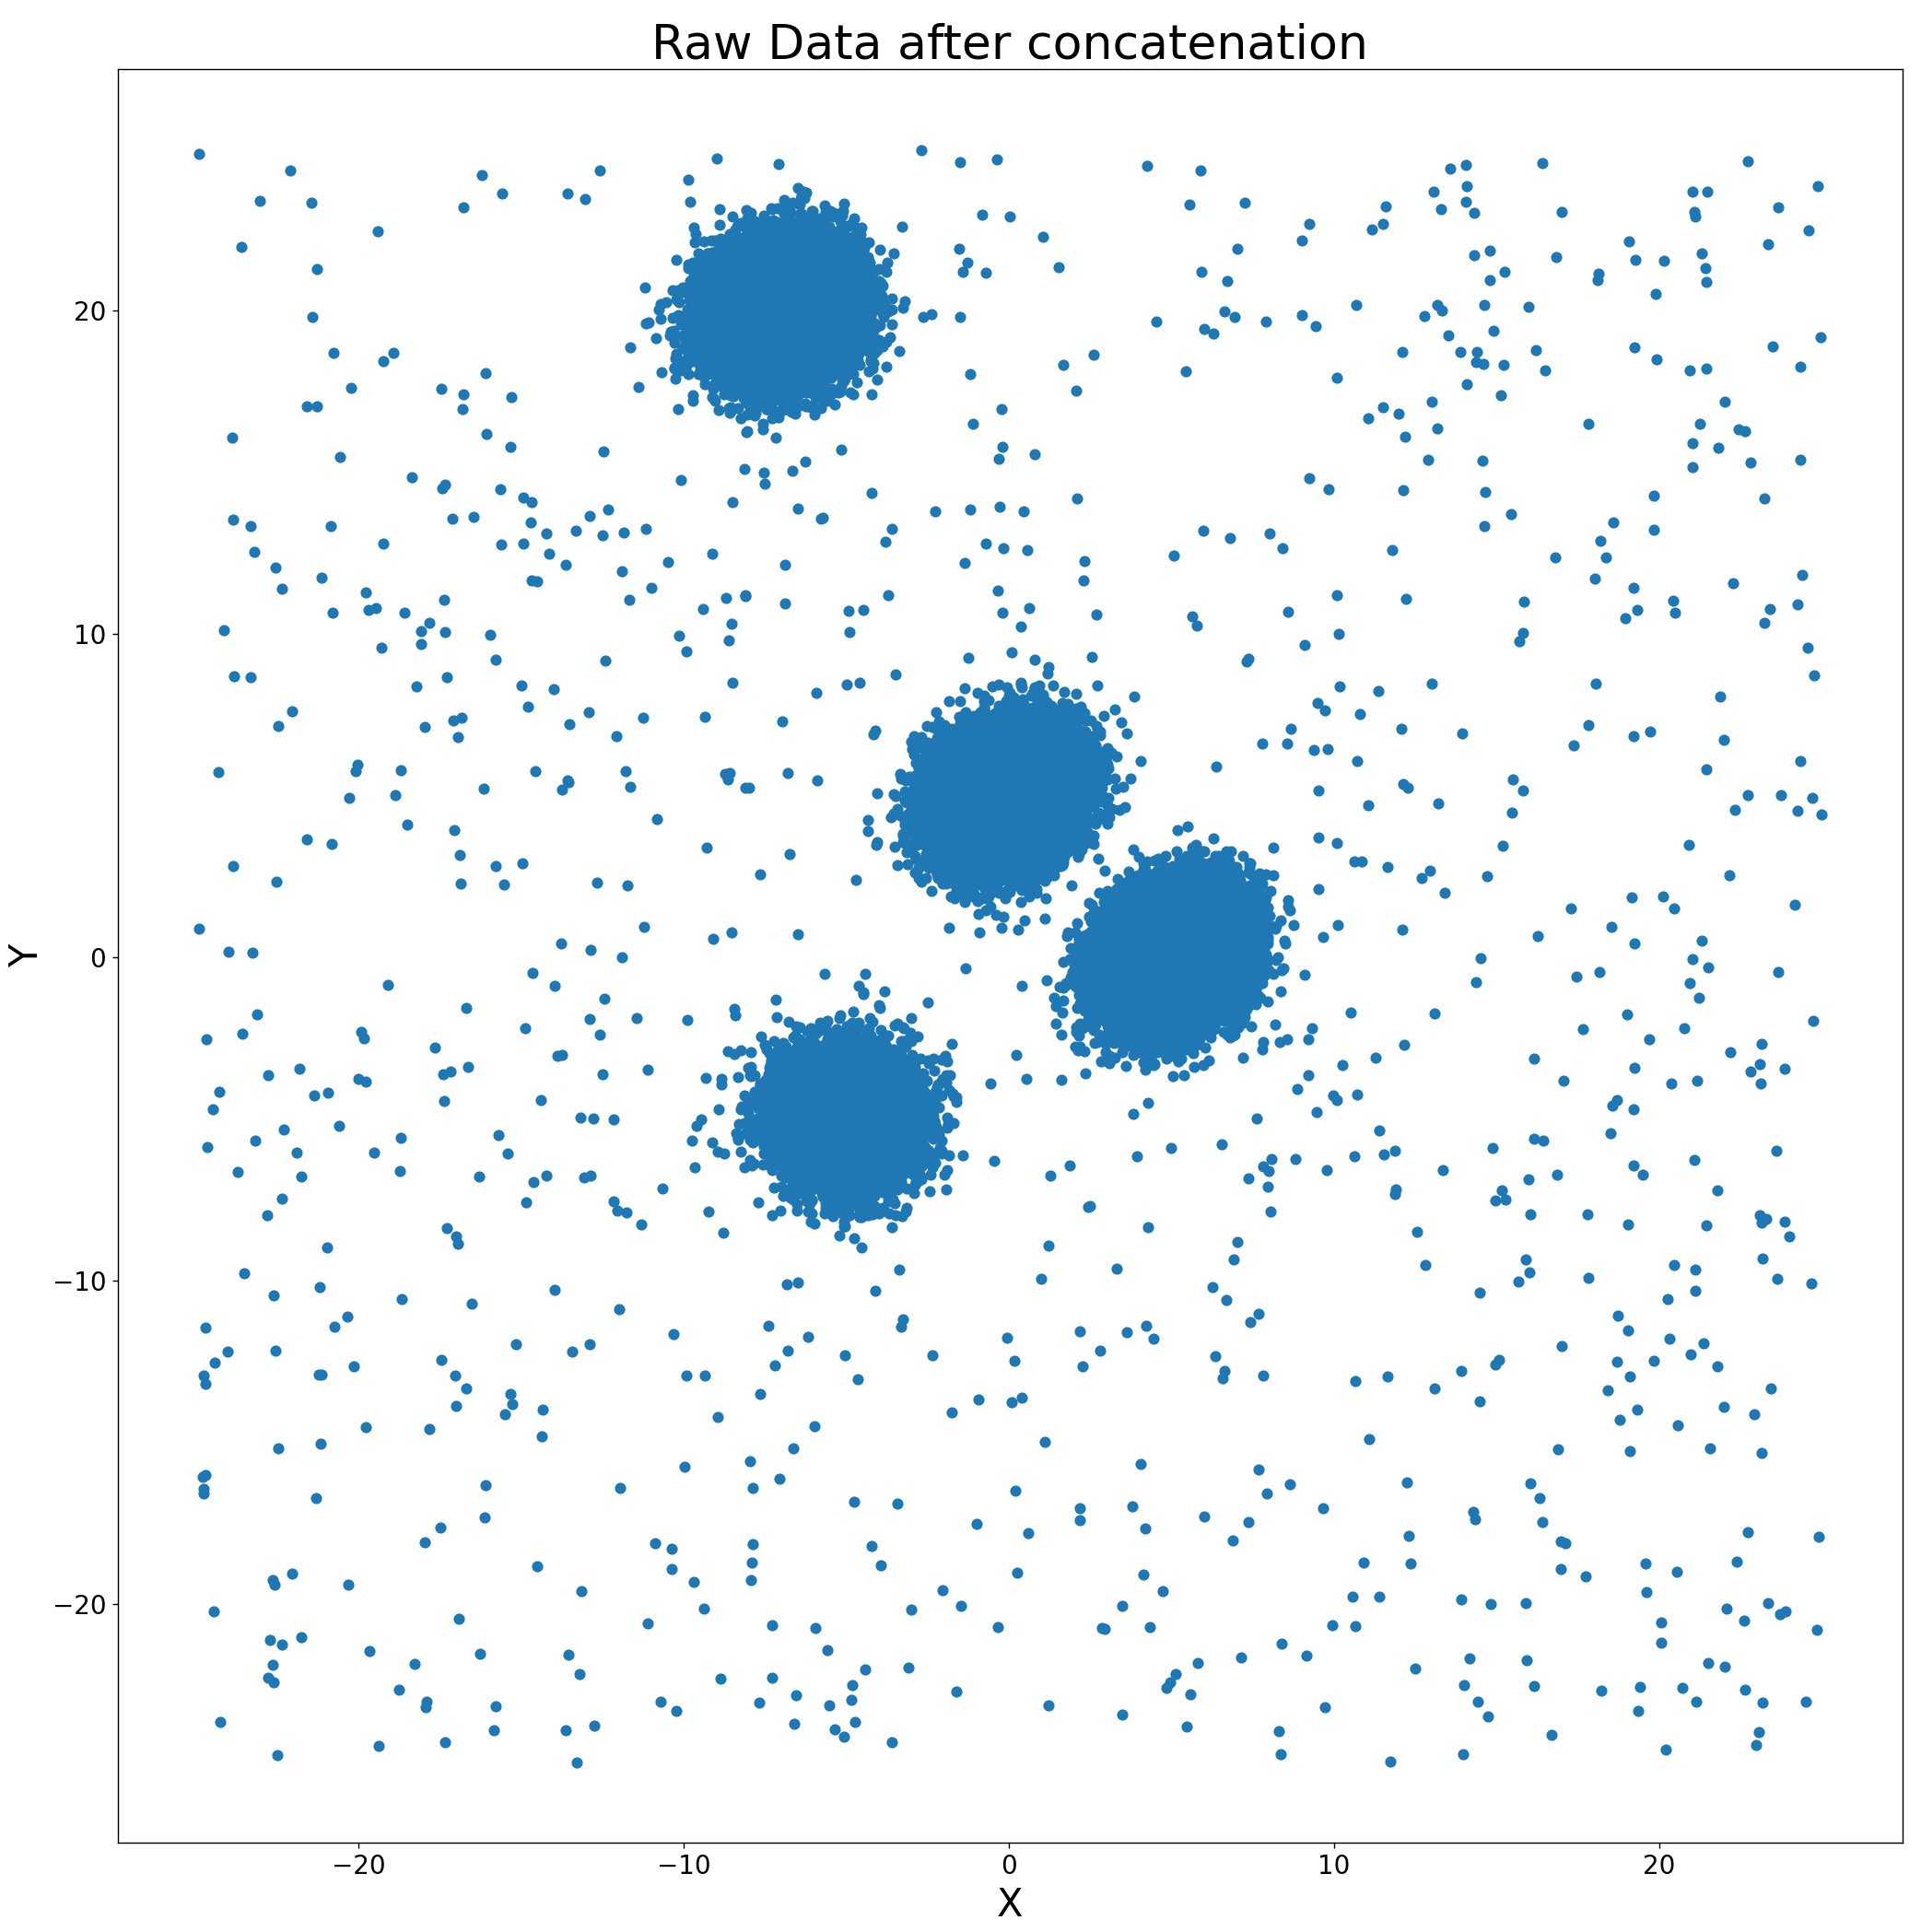
\includegraphics[width=0.5\textwidth]{2d_img0.png}
    \caption{Raw 2-d data}
    \label{fig:2d_raw}
\end{figure}

\begin{figure}[H]
    \centering
    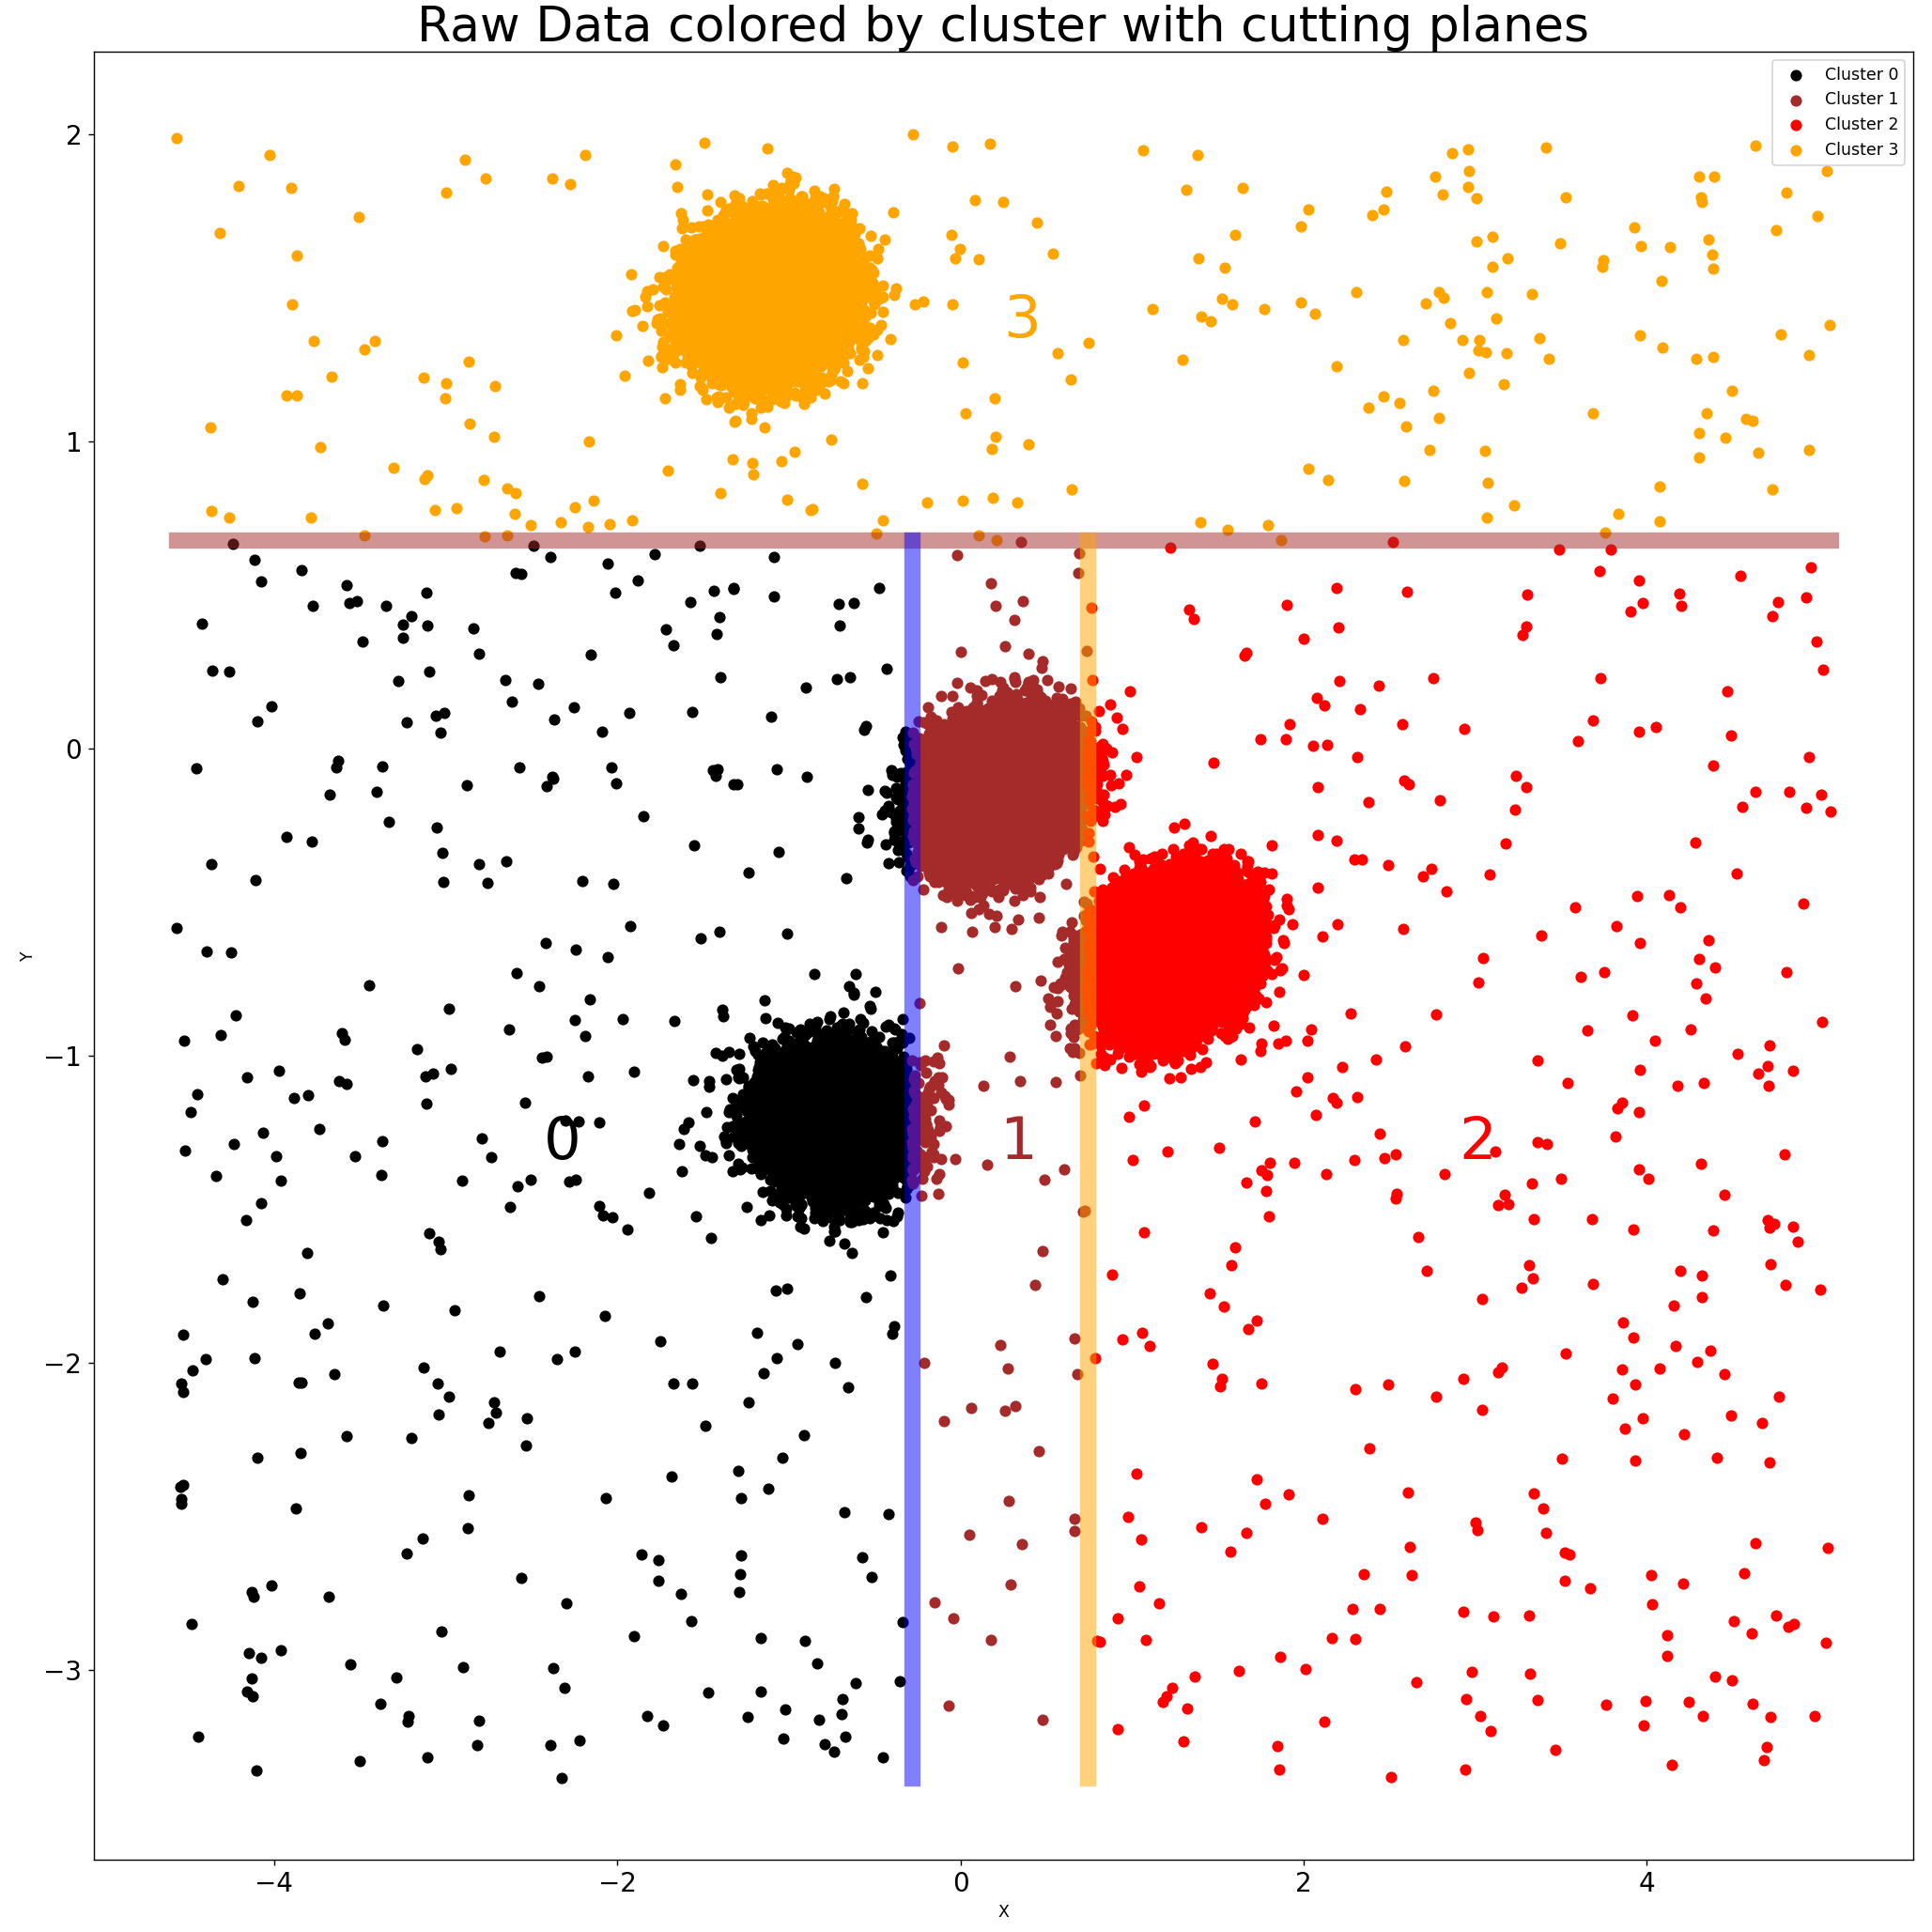
\includegraphics[width=0.5\textwidth]{2d_img1.png}
    \caption{Clustered 2-d data}
    \label{fig:2d_clustered}
\end{figure}

The  raw data is shown in Figure \ref{fig:2d_raw} and the clustered data is shown in Figure \ref{fig:2d_clustered}. 
In the labelled figure, you can see the clusters are labelled by grid location and colored using the resistor color code. The noise is shown in the figure to show how it interacts with the grid.
Adding the noise was critical to debug the grid line locations.\par
The algorithm chose two cutting planes in the bottom half that did not do a very good job of splitting the clusters. Also, the grid nature of the algorithm is on display with the interaction of cluster 1 with cluster 0 and cluster 2.
\subsection{3-d results}
In this section, we will present the results of the 3-d data. The following graphs will display the labelled cluster data and various views of the 3-d data.  The clustered data is shown in Figure \ref{fig:3d_clustered}.
The clusters were generated with a couple of functions that first generate a grouping of cluster centers then populates the cluster centers based on a number of parameters.\par
Optigrid settings: 7 Clusters, up to 1000 points per cluster, up to sigma of 2.0, $kde\_bandwidth$ of 0.1, $noise\_level$ of 0.1, max cut score of 0.3

\begin{tcolorbox}
    \small
Cluster 0: Mean=[ 0.35 -1.49 -1.08], Std=[0.17 0.17 0.35]\newline
Cluster 1: Mean=[-0.53 -0.31 -0.77], Std=[0.20 0.26 0.33]\newline
Cluster 2: Mean=[-1.36   0.83 -0.72], Std=[0.05 0.05 0.06]\newline
Cluster 3: Mean=[-1.97 -1.98  1.14], Std=[0.06 0.09 0.11]\newline
Cluster 4: Mean=[0.41 0.56 1.13], Std=[0.14 0.18 0.23]\newline
Cluster 5: Mean=[1.22 0.68 0.98], Std=[0.04 0.06 0.07]
\end{tcolorbox}
\normalfont

\begin{figure}[H]
    \centering
    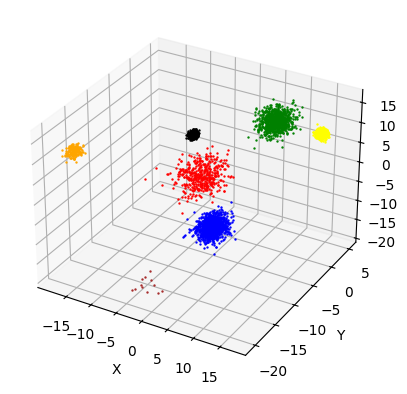
\includegraphics[width=0.5\textwidth]{3d_cluster_raw.png}
    \caption{Clustered 3-d data}
    \label{fig:3d_clustered}
\end{figure}

The upcoming images will show the results of OptiGrid clustering. The first three images in the series will provide planar perspectives, while the next images will show other various perspectives.

\begin{figure}[H]
    \centering
    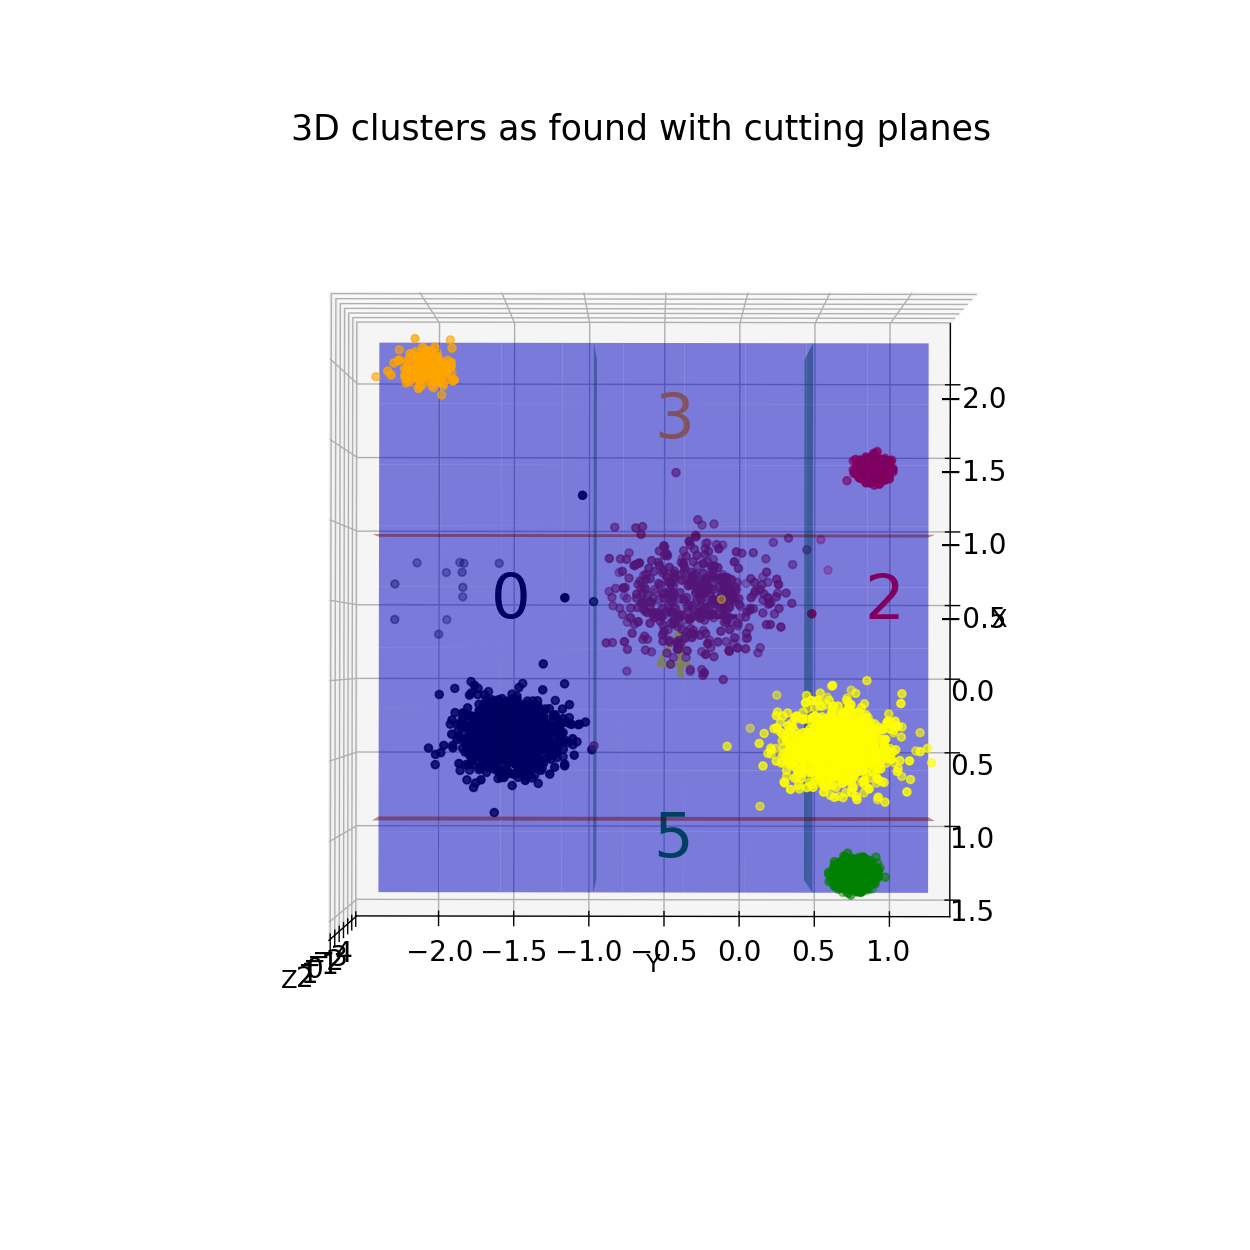
\includegraphics[width=0.5\textwidth]{3d_img_xy.png}
    \caption{XY plane perspective of 3-d data}
    \label{fig:3d_cluster_0}
\end{figure}

\begin{figure}[H]
    \centering
    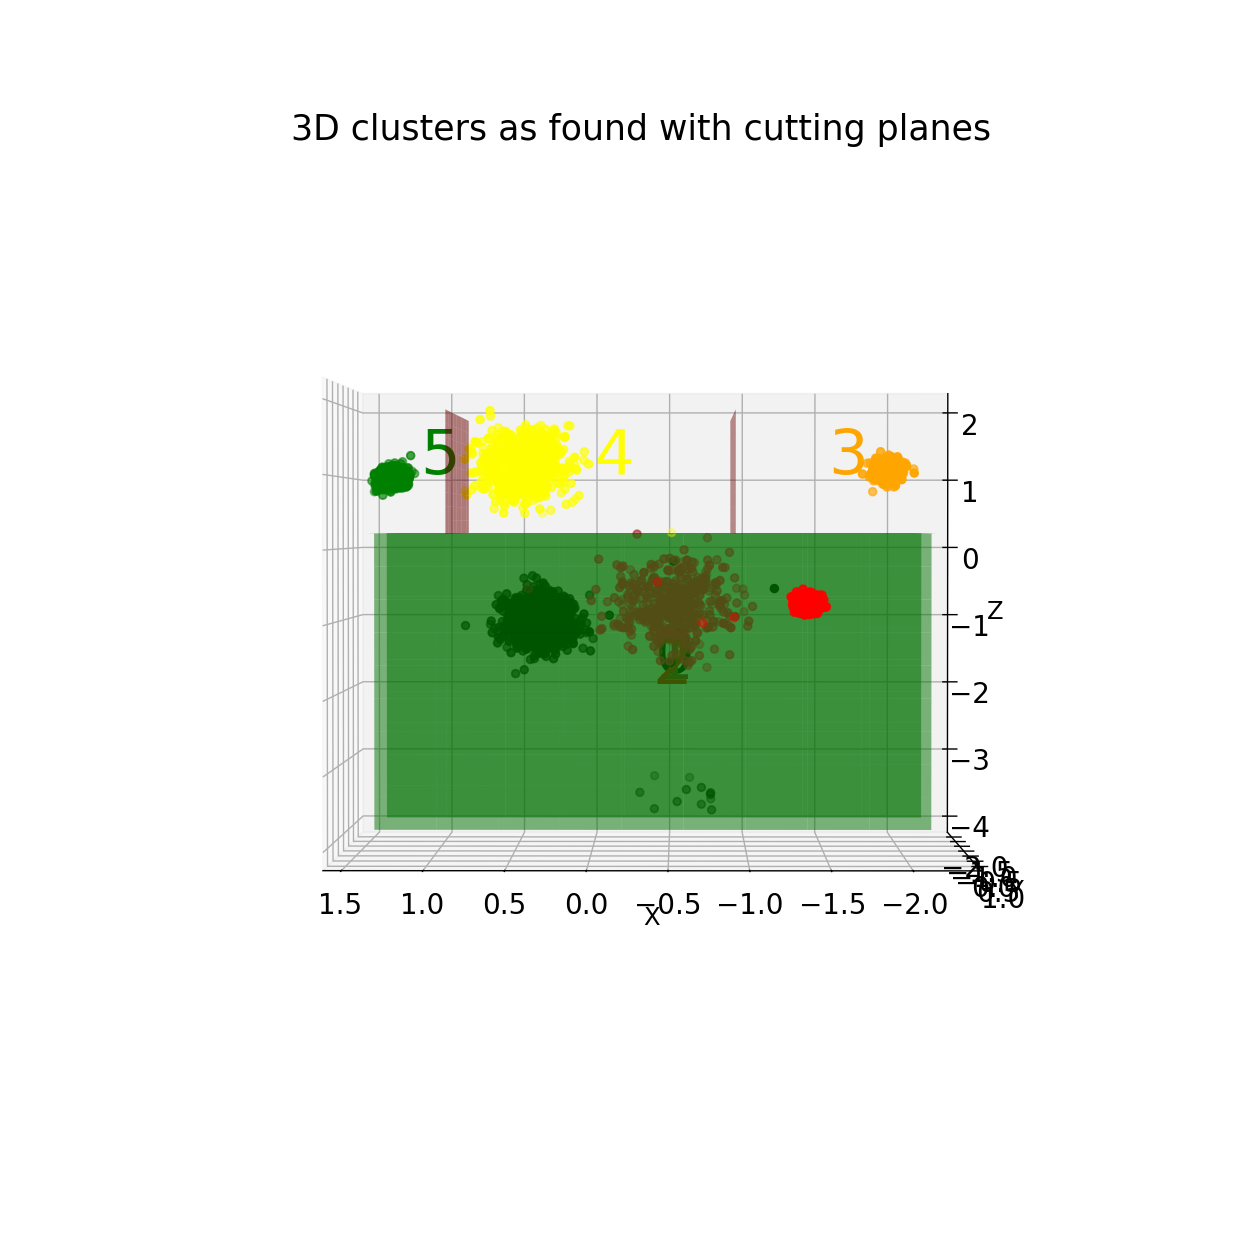
\includegraphics[width=0.5\textwidth]{3d_img_xz.png}
    \caption{XZ plane perspective of 3-d data}
    \label{fig:3d_cluster_1}
\end{figure}

\begin{figure}[H]
    \centering
    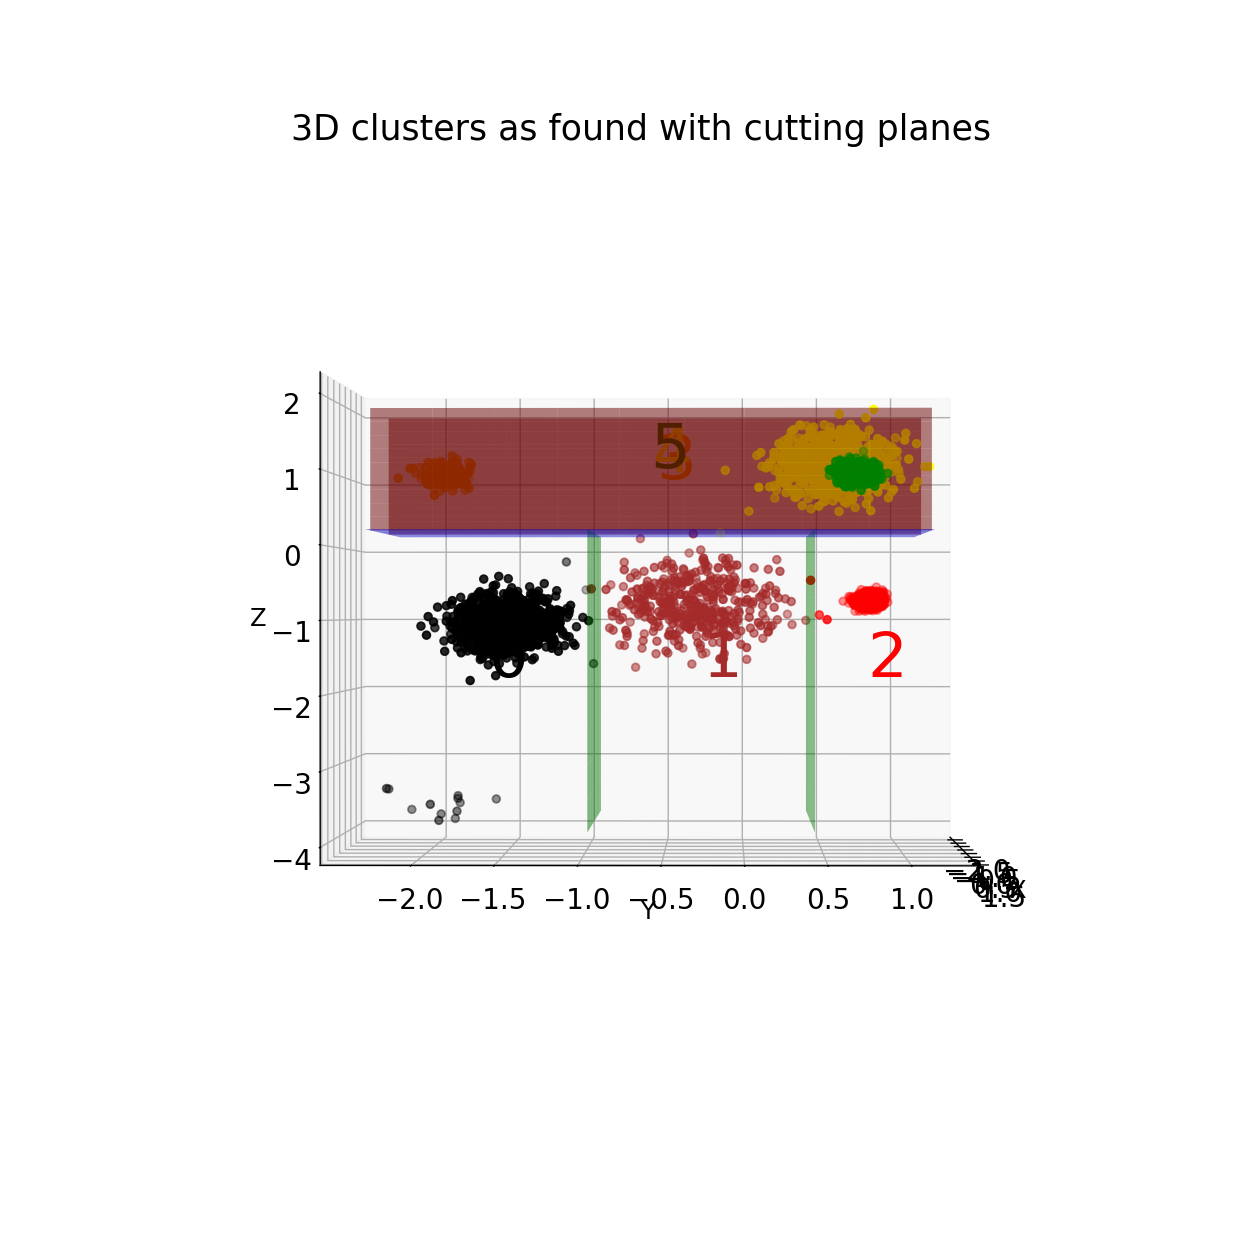
\includegraphics[width=0.5\textwidth]{3d_img_yz.png}
    \caption{YZ plane perspective of 3-d data}
    \label{fig:3d_cluster_2}
\end{figure}

\begin{figure}[H]
    \centering
    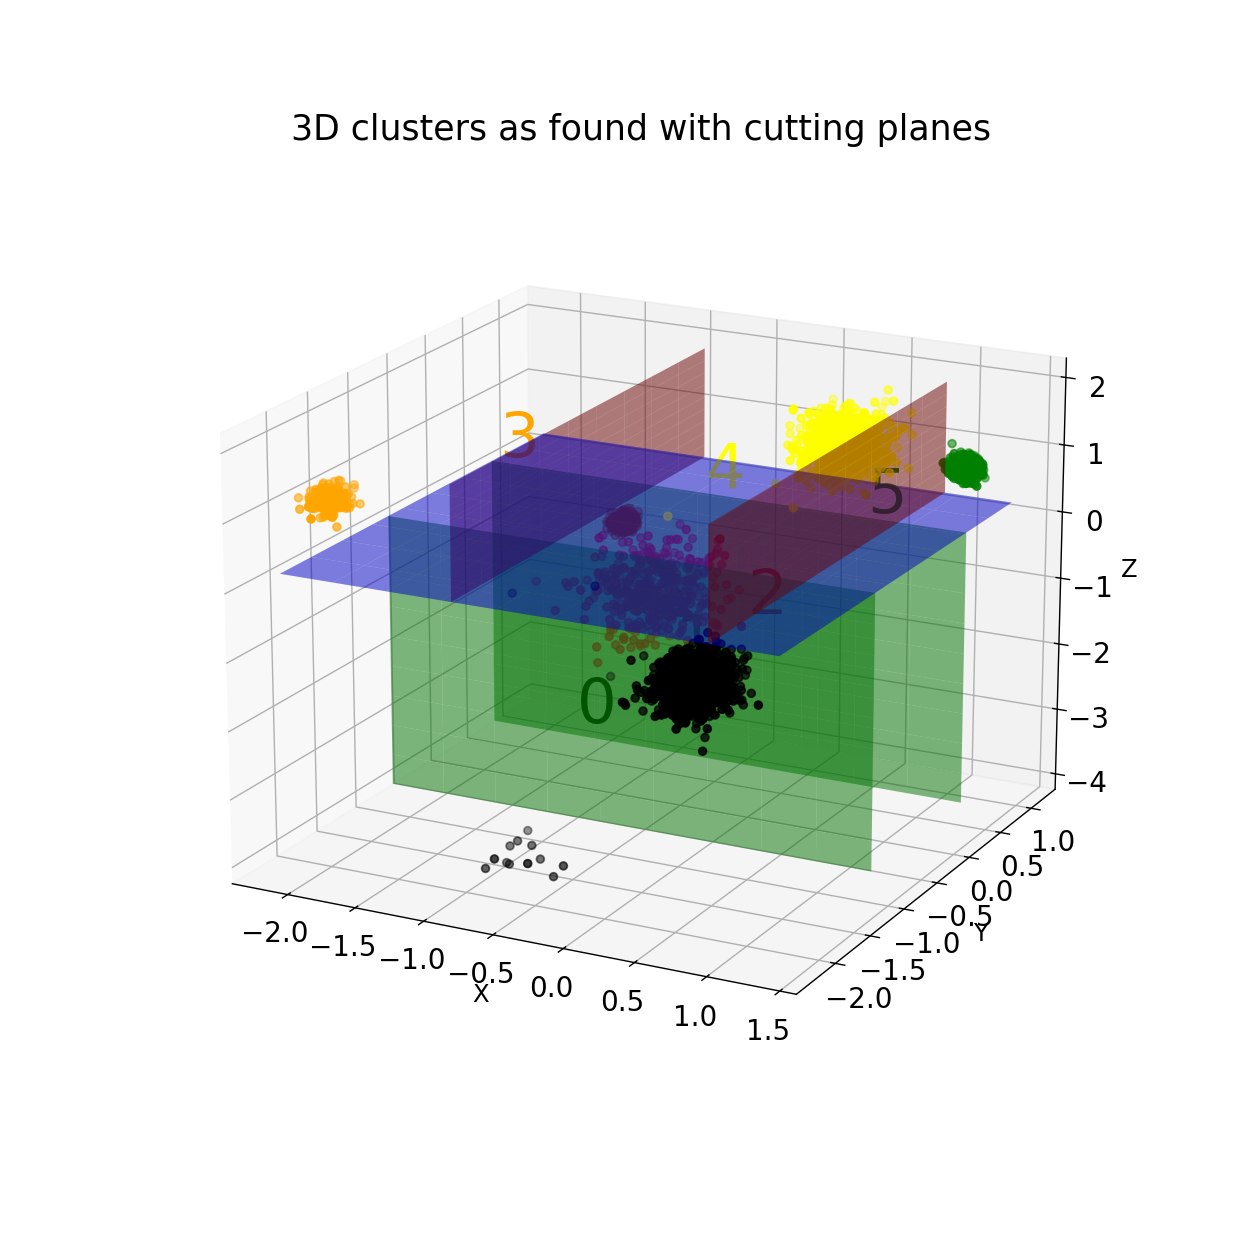
\includegraphics[width=0.5\textwidth]{3d_img1.png}
    \caption{Perspective 1 of 3-d data}
    \label{fig:3d_cluster_3}
\end{figure}

\begin{figure}[H]
    \centering
    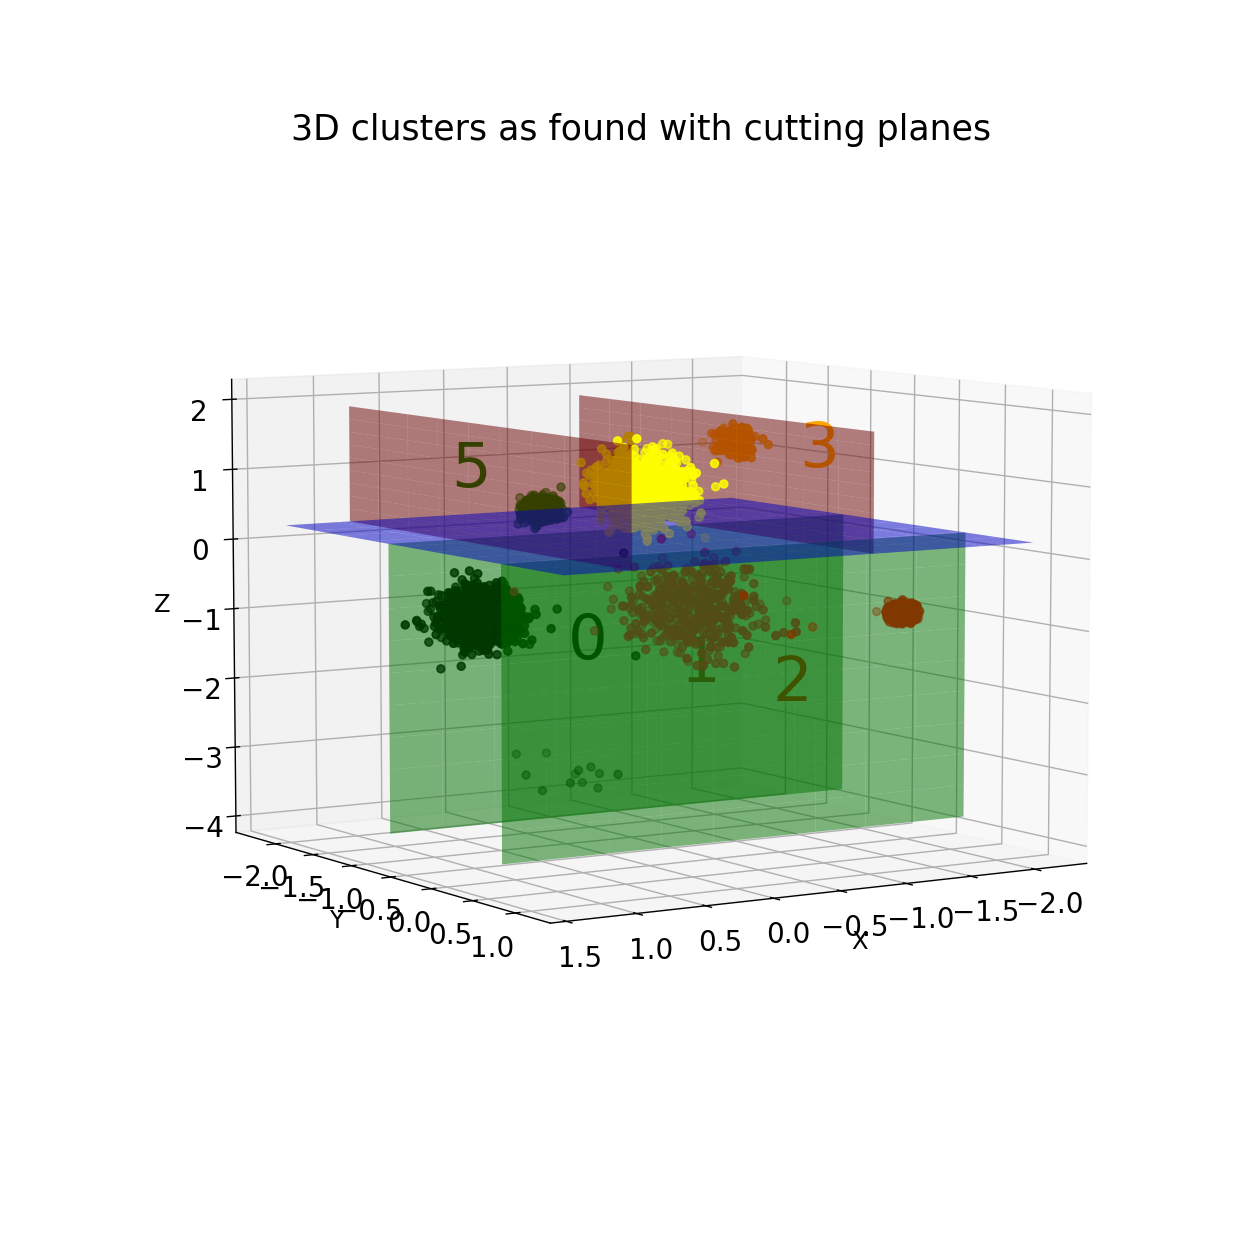
\includegraphics[width=0.5\textwidth]{3d_img3.png}
    \caption{Perspective 2 of 3-d data}
    \label{fig:3d_cluster_4}
\end{figure}
